\section{Introduction}
Over the last seven years, Florida's Coral Reef (FCR) has suffered from a widespread decline in living, reef-building corals due to a multi-year coral-disease outbreak \citep{precht2016unprecedented,walton2018impacts}, called stony coral tissue loss disease (SCTLD). First reported off the coast of Miami-Dade county in 2014, the disease has since spread through the entirety of FCR as well as other sites within the Caribbean \citep{alvarez2019rapid,kramer2019map,estrada2020reef} and affected more than 20 scleractinian coral species \citep{noaa2018}. The range of species affected coupled with the large spatial and temporal extents of the outbreak make SCTLD the most severe disease outbreak to have affected coral reefs on record.

Previous study of the spatio-temporal dynamics of SCTLD between West Palm Beach and Marathon showed that the epizootic propagated at a rate of $\sim$100 m/day to the north and $\sim$92 m/day to the south, hitting the Middle Florida Keys in 2017 \citep{muller2020spatial}. The disease was then reported in the Lower Keys in summer 2018 \citep{frrp2018}; near Key West in winter 2018 \citep{frrp2018}; on the easternmost boundary of the Marquesas subregion in October 2019 \citep{frrp2019}; and at its western end, approximately 11 km west of halfmoon shoal, in August 2020 \citep{frrp2020}. SCTLD was observed propagating faster than 100 m/day within the Marquesas between October 2019 and August 2020 and would have reached the reefs of the Dry Tortugas (DRTO) by February 2021 if it had spread at a similarly high propagation rate \citep{kramer2019map}. These propagation rates were observed in a relatively dense shallow-water reef system and mostly occurred through transmission from neighbor to neighbor. Disease agents then had to cross 30 km ($\sim$20 miles) of open waters to reach the reefs of the DRTO. The disease was ultimately observed in May 2021 \citep{kramer2019map} in the southeast of the DRTO. To date, questions remain about the timing of the spread of the disease to the DRTO as well as the role played by hydrodynamics in the process.

The DRTO coral reefs are among the most preserved, but also vulnerable, marine ecosystems of the continental United States \citep{kourafalou2018physical}. They are part of the Florida Keys National Marine Sanctuary (FKNMS), under the jurisdiction of the Tortugas Ecological Reserve that covers around 566 km$^2$ of no-take marine reserves \citep{ault2006building}. Since the establishment of DRTO in July 2001, fish populations within the managed areas have significantly increased in size, adult abundance, and occupancy rates, therefore favoring the establishment of sustainable fisheries \citep{ault2013assessing}. Furthermore, because of their location and hydrodynamics, DRTO reefs are believed to be important sources of recruitment for coral-reef fishes downstream in the Florida Keys \citep{domeier2004potential} and thus significantly contribute to the overall resilience of the Florida Keys coral-reef ecosystem.

Although the pathogen responsible for the disease remains unknown to date, hydrodynamics are likely to play an important role in its propagation. Modeling studies suggest that the observed spread of the disease can be reproduced by simulating the dispersal of neutrally buoyant particles \citep{dobbelaere2020coupled}, while ex situ experiments show evidence of waterborne disease transmission \citep{aeby2019pathogenesis, eaton2021measuring,meiling2021variable}. Accounting for the underlying ocean circulation is therefore important to understand the evolution of the propagation of the disease. The observed apparent stalling of the spread of SCTLD from the Marquesas to DRTO reefs may be explained by ephemeral or persistent oceanographic features in the area that initially prevented the transmission of disease agents further west.

The ocean circulation between the Marquesas and the DRTO is strongly driven by the Loop Current (LC). This ocean current brings warm waters from the Caribbean Sea through the Yucatan Channel, loops anti-cyclonically through the northeastern Gulf of Mexico (GoM) and finally exits through the southern Straits of Florida, where it forms the Florida Current (FC). The northward penetration of the LC through the GoM varies throughout the year, and sporadically an anticyclonic ring separates from the current \citep{leipper1970sequence, maul1977annual,vukovich1988loop}. The dominant mesoscale feature near the DRTO is the formation of quasi-stationary eddies with a diameter of 100-200 km \citep{lee1994evolution,fratantoni1998influence}, usually called Tortugas gyres or eddies. \cite{fratantoni1998influence} hypothesized that the formation of these eddies as well as their lifespan was linked to the generation of anticyclonic rings from the LC in the GoM, while \cite{kourafalou2012florida} showed the relation between eddy formation dynamics near the DRTO and meandering of the FC. These eddies can remain up to 120 days near the DRTO before moving eastward at a speed of 5 km/day under the action of LC frontal eddies \citep{maul1977annual}. Tortugas gyres have been identified as an important mechanism for the potential retention of larvae of invertebrates and fishes on the southwest Florida shelf \citep{lee1994evolution, sponaugle2005florida, kourafalou2012florida} and might therefore have impacted the dispersal of disease agents from the Marquesas to the DRTO.

The objective of the present study was to apply the same modeling tools as \cite{dobbelaere2020coupled} to determine the potential impact of the circulation in the GoM on the delayed propagation of SCTLD between the Marquesas and the DRTO. This was performed by evaluating the evolution of the hydrodynamic-predicted connectivity between these two regions between May 2018 and May 2021. We then assessed how large-scale ocean circulation features, such as Tortugas gyres, could have prevented the transport of potential disease agents from the Marquesas to the DRTO. Ultimately, this study aims to provide novel insight on the role hydrodynamics have played in the spread of SCTLD throughout the western-most area of FCR, which further informs how it has, and will continue to, spread throughout the tropical western Atlantic

% === METHODS === %
\section{Methods}
Stony Coral Tissue Loss Disease data was obtained by using the Florida Reef Resilience Program's Disturbance Response Monitoring Report for 2019 and 2020 \citep{frrp2019,frrp2020} as well as the Atlantic and Gulf Rapid Reef Assessment (AGGRA) resources for SCTLD reported throughout the Caribbean, an open access spatial and temporal database curated by experts in Caribbean coral reef ecology \citep{kramer2019map}. Assumptions associated with SCTLD included the following: (\textit{i}) SCTLD is different from other tissue loss diseases previously reported on corals (i.e. white plague, white syndrome) based on its ecology and case definition \citep{noaa2018}, (\textit{ii}) SCTLD is transmitted, in part, by ocean currents \citep{aeby2019pathogenesis, muller2020spatial,eaton2021measuring} and (\textit{iii}) SCTLD was along the western most reef area of the Lower Florida Keys in October 2019, reached the western most part of the Marquesas in August 2020, and did not occur in DRTO until May 2021 based on curated data provided by the FRRP reports and the AGGRA open access database.

We studied the transmission patterns of SCTLD between the Marquesas and the DRTO by using the hydro-epidemiological model of \cite{dobbelaere2020coupled}. This model relies on the multi-scale ocean model SLIM\footnote{\url{ https://www.slim-ocean.be}} to simulate the hydrodynamics over the entirety of FCR. The computational domain includes the Florida Straits as well as part of the GoM (Fig. \ref{fig:fig1_drto}a). SLIM is coupled with the large-scale ocean model HYCOM in order to correctly represent the dynamics of the FC which is a major western boundary current that flows out of the GoM, as a continuation of the Loop Current, before joining the Gulf Stream. SLIM uses an unstructured mesh whose resolution can be locally increased in order to accurately represent fine-scale flow features. Here we used the same mesh as \cite{dobbelaere2020coupled}, composed of $7\times 10^5$ elements, and with resolution that reaches 100 m over reefs and along the coastline (Fig \ref{fig:fig1_drto}a). By using such a fine resolution, we can explicitly represent circulation and resolve tides at the reef scale, such as around the Marquesas island group (Fig. \ref{fig:fig1_drto}a, inset), while also representing the large-scale flow features within the FC (Fig 1b and c). Further details on the model are provided by \cite{frys2020fine}. \modif{The model results were validated against tide gauge and ADCP measurements and showed good agreement with observations (see appendix \ref{drto:validation})}.

\begin{figure}
    \centering
    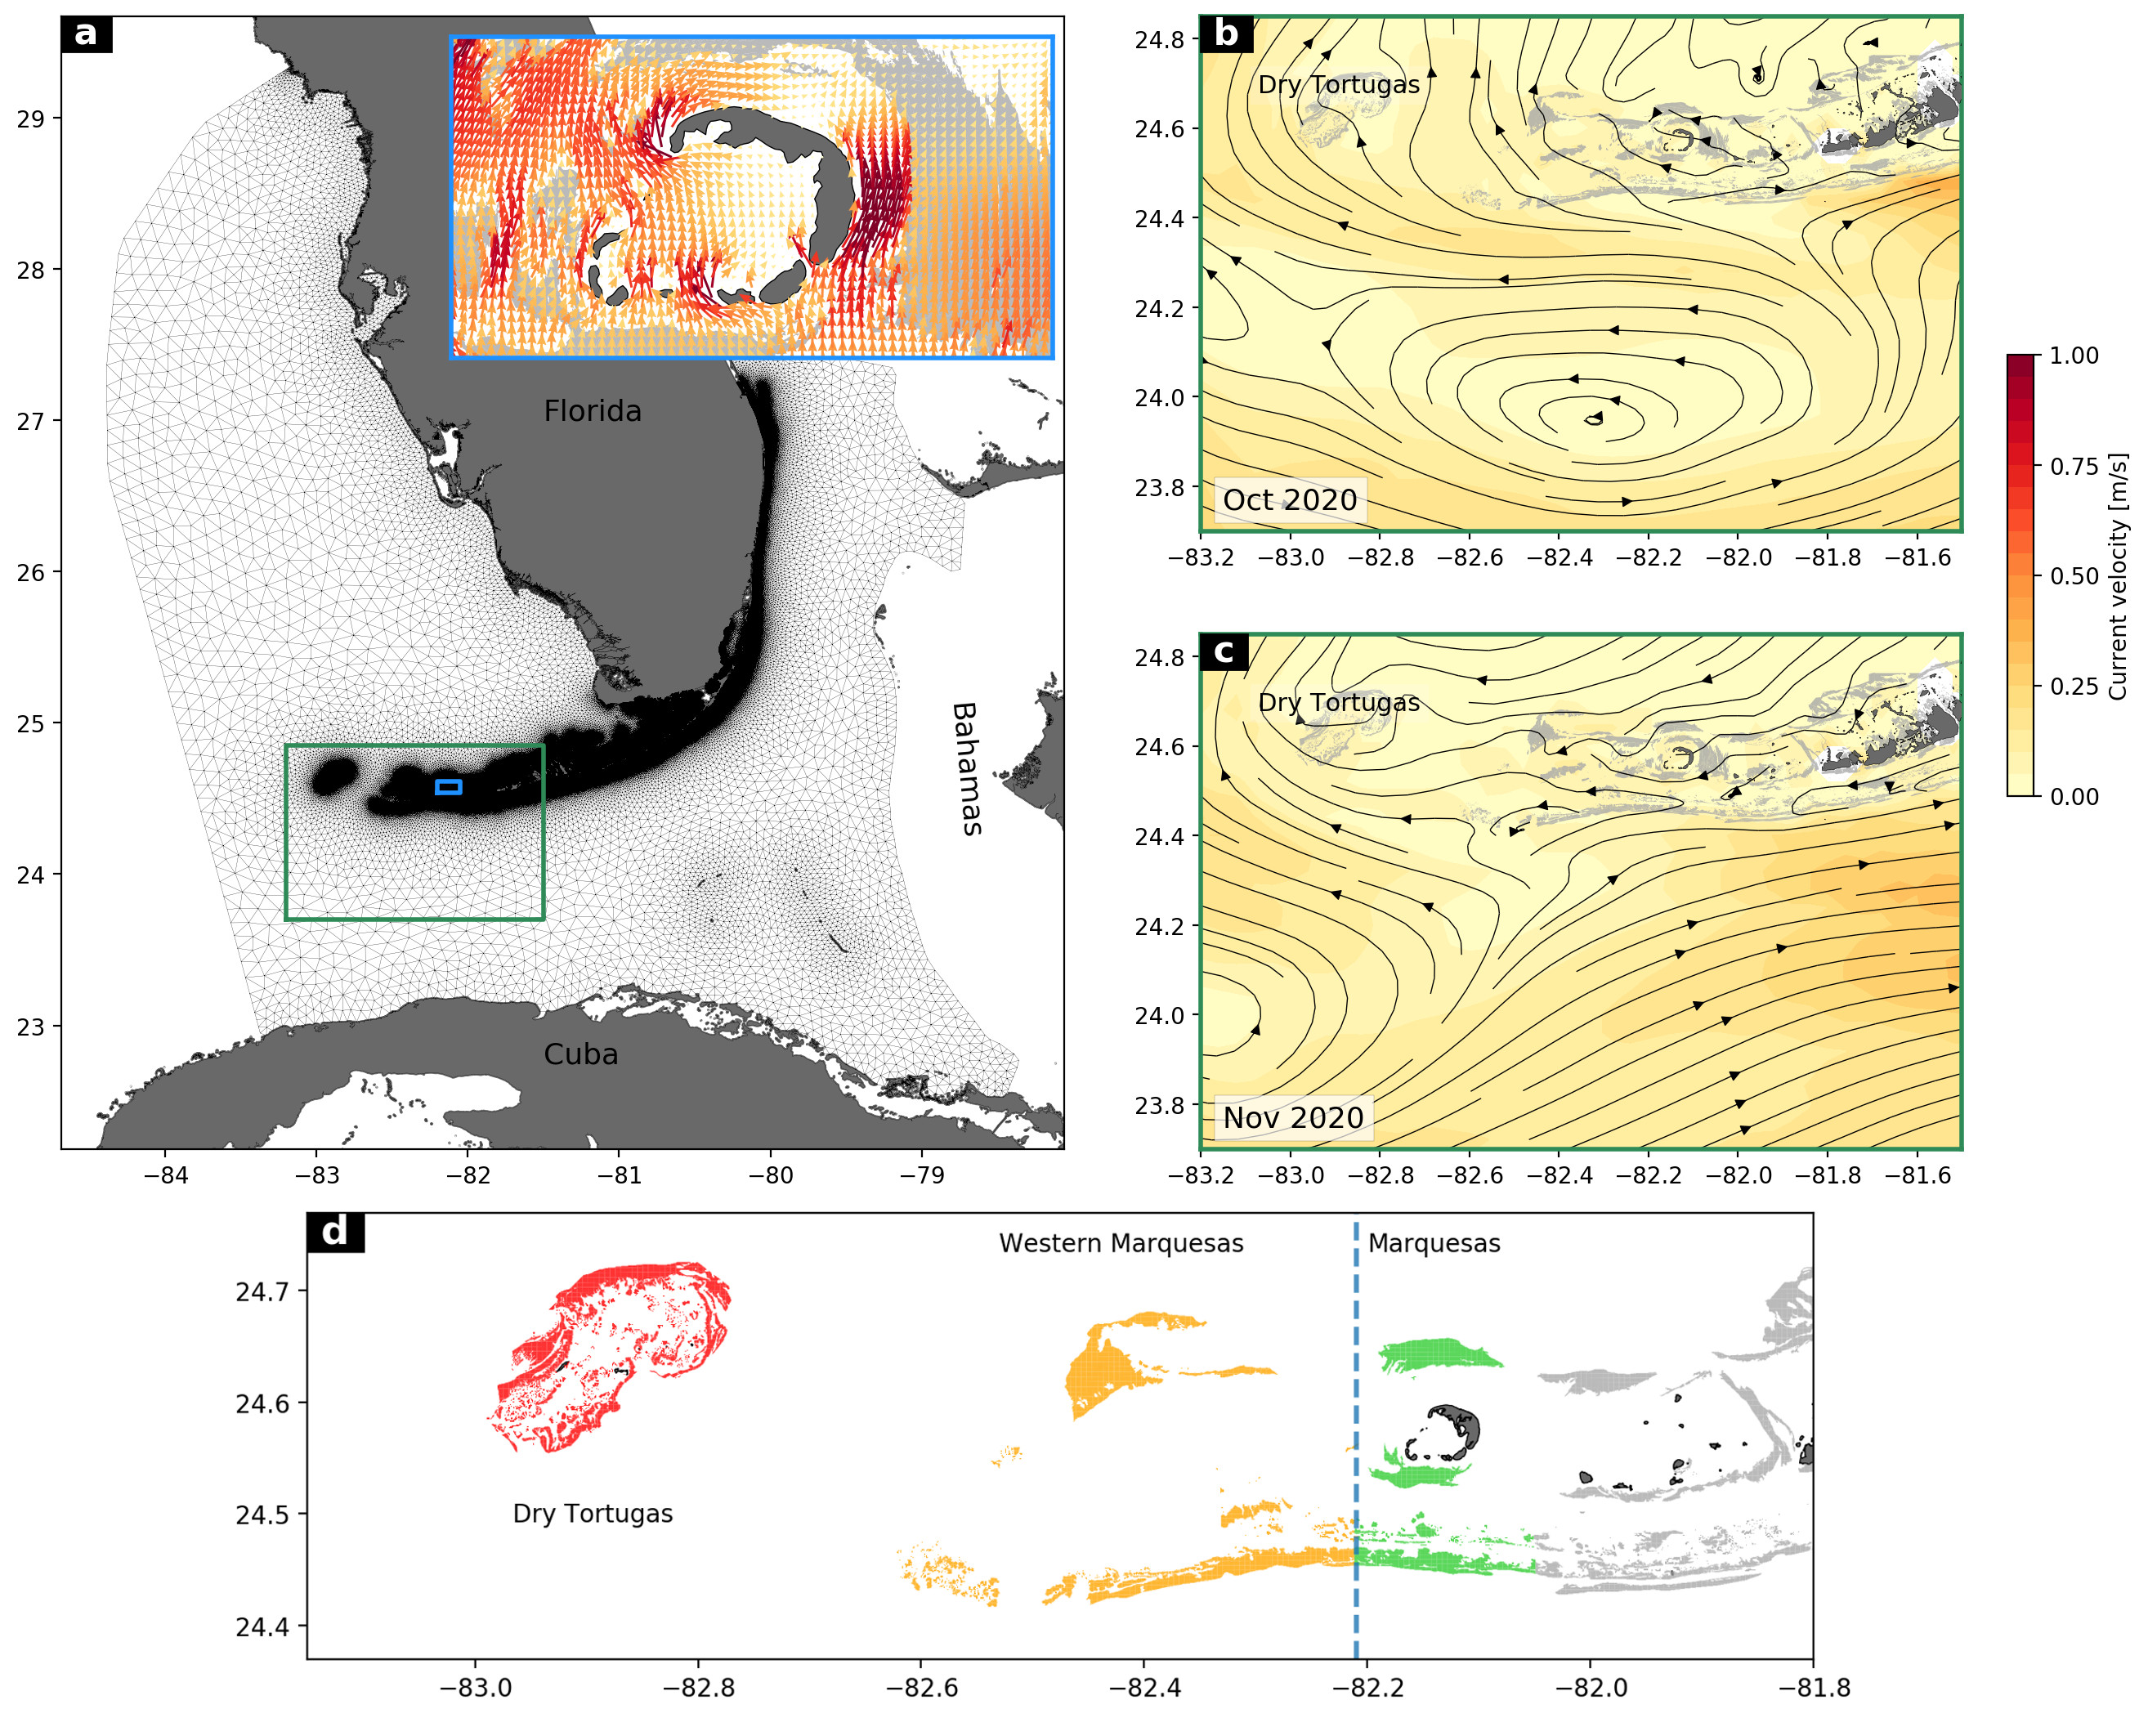
\includegraphics[width=.95\textwidth]{chapters/drto/figures/fig1.jpg}
    \caption{(a) Mesh of the computational domain and close-up view of the instantaneous currents on November 15, 2020 at 12:00 in the Marquesas (inset), (b) close-up view of the monthly-averaged circulation between the Marquesas and the DRTO in October 2020, and (c) November 2020. (d) Reefs of the areas of the DRTO, the Western Marquesas and the Marquesas, as defined in this study. Land is shown in dark gray and reefs in light gray, except in panel (d) where reefs from the Marquesas, the Western Marquesas and the DRTO are respectively shown in green, yellow and red. Streamlines indicate the presence of the Tortugas gyre in October 2020, which leads to northward currents between the Marquesas and the DRTO. In November, the gyre left its static location to transit through the Straits of Florida and currents between the Marquesas and DRTO became westward.}
    \label{fig:fig1_drto}
\end{figure}

We simulated the dispersal of disease agents throughout FCR between May 2018 and May 2021. As in \cite{dobbelaere2020coupled}, disease agents were modeled as passive particles transported by depth-averaged currents which constantly lost mass with a half-life of 30 days. We ran the particle transport model for every month between May 2018 and May 2021 and hence obtained monthly normalized connectivity matrices. An entry $C_{ij}$ of the connectivity matrix represents the probability that disease agents produced on sub-reef $i$ settle on sub-reef $j$. These sub-reefs were defined by extracting polygons from the “coral reefs and hard bottom” layer of the Unified Florida Reef Tract Map \citep{fwc2017unified} and further dividing them into 500 m $\times$ 500 m squares, generating a total of 16,823 sub-reef polygons. Since the connectivity matrices had more than 200 million entries, they were not directly interpreted. Instead, they were represented as large networks where nodes corresponded to sub-reefs of FCR and edges corresponded to nonzero entries in the connectivity matrix. Graph-theory algorithms were then used to analyze the properties of the connectivity networks. 

To quantify the connectivity between the Marquesas and the DRTO, we defined 3 sub-regions within the sub-reefs of the western part of FCR: (\textit{i}) the Marquesas, (\textit{ii}) the Western Marquesas and (\textit{iii}) the DRTO (Fig. \ref{fig:fig1_drto}d). The sub-region of the Marquesas was defined as all the sub-reefs whose centroid is located between $-82.21^\circ$ and $-82.05^\circ$ longitude; the Western Marquesas included all sub-reefs between $-82.73^\circ$ and $-82.21^\circ$; and the DRTO were composed of  all the sub-reefs in our domain located west of $-82.73^\circ$ longitude. We evaluated the exchanges between two given sub-regions by identifying all edges connecting any sub-reef from one sub-region to any sub-reef from the other sub-region in our monthly connectivity networks. We then defined a connectivity indicator by multiplying the number of these direct edges by their mean connection probability. This indicator was computed monthly between May 2018 and May 2021 to evaluate the connectivity (\textit{i}) from the Marquesas to the DRTO, (\textit{ii}) from the Western Marquesas to the DRTO and (\textit{iii}) from the Marquesas to the Western Marquesas.

The spatial information of the network can be used to predict which part of the DRTO was likely to be first exposed to potential disease agents via hydrodynamic connections. We built a monthly spatial vulnerability indicator by summing the probabilities of all edges connecting sub-reefs of the Marquesas and the Western Marquesas to a given sub-reef of the DRTO. Sub-reefs of the DRTO with larger values of this indicator would have a larger cumulative likelihood of being infected during the simulated month. Such areas would thus be more likely to be the "entry points" of SCTLD in the DRTO during the month, as they were the destination of more pathways with larger exchange probabilities. A similar indicator can be computed for the Marquesas and the Western Marquesas by summing the probabilities of the edges connecting a given sub-reef of these sub-regions to the DRTO. Sub-reefs with higher value of this source indicator would be more likely to initiate the propagation of the disease to the DRTO, as they were the origin of more connectivity pathways with larger exchange probabilities. Model predictions were then compared to actual observations of the first cases of SCTLD in the DRTO collected on the interactive map of \cite{kramer2019map}. 

To understand the effect of the ocean circulation on disease transmission, we computed the monthly-averaged circulation for each simulated month. These residual currents were used to visually assess the presence of a Tortugas gyre during that month, i.e. the presence of eastward moving eddies persisting on temporal and spatial scales consistent with the description of \cite{lee1994evolution} in the vicinity of the DRTO. Moreover, we defined an axis from the Marquesas to the DRTO over which we averaged the monthly residual currents. These temporally and spatially averaged currents were used as a proxy of the circulation between the Marquesas and the DRTO during each simulated month.

\section{Results}
The evolution of the monthly connectivity indicator suggests that there were no exchanges from the Marquesas and the Western Marquesas to the DRTO between February and October 2020, and between January and May 2021 (Fig. \ref{fig:fig2_drto}a). This is quite remarkable as outside of these periods of low connectivity, there were no periods greater than four months without exchange from both the Marquesas and the Western Marquesas between May 2018 and May 2021. Furthermore, February-October 2020 and March 2021 were the only months characterized by mean currents with an eastward component between the Marquesas and the DRTO (Fig. \ref{fig:fig2_drto}b). These periods of low connectivity and circulation inversion appeared correlated with the presence of eddies near the DRTO, as Tortugas gyres were observed during most months with no simulated connections to the DRTO. Additionally, no exchange occurred in September 2019 or from January to February 2021, during which a strong southward mean circulation occurred between the Marquesas and the DRTO (Fig. \ref{fig:fig2_drto}b). This suggests that southward currents might also act as a barrier to disease propagation by flushing away disease agents south to the GoM. Connectivity from the Marquesas to the Western Marquesas was never completely interrupted during our simulated period (Fig 2a). Nonetheless, periods of low connectivity to the DRTO occurred in the presence of Tortugas eddies (April-June 2020) and southward circulation (February 2021). This suggests that propagation of disease agents from the Marquesas to the Western Marquesas was routinely possible, even though exchanges may have been hindered by the local circulation. This latter result is consistent with the observed westward propagation of the disease in the Marquesas between October 2019 and August 2020.

\begin{figure}
    \centering
    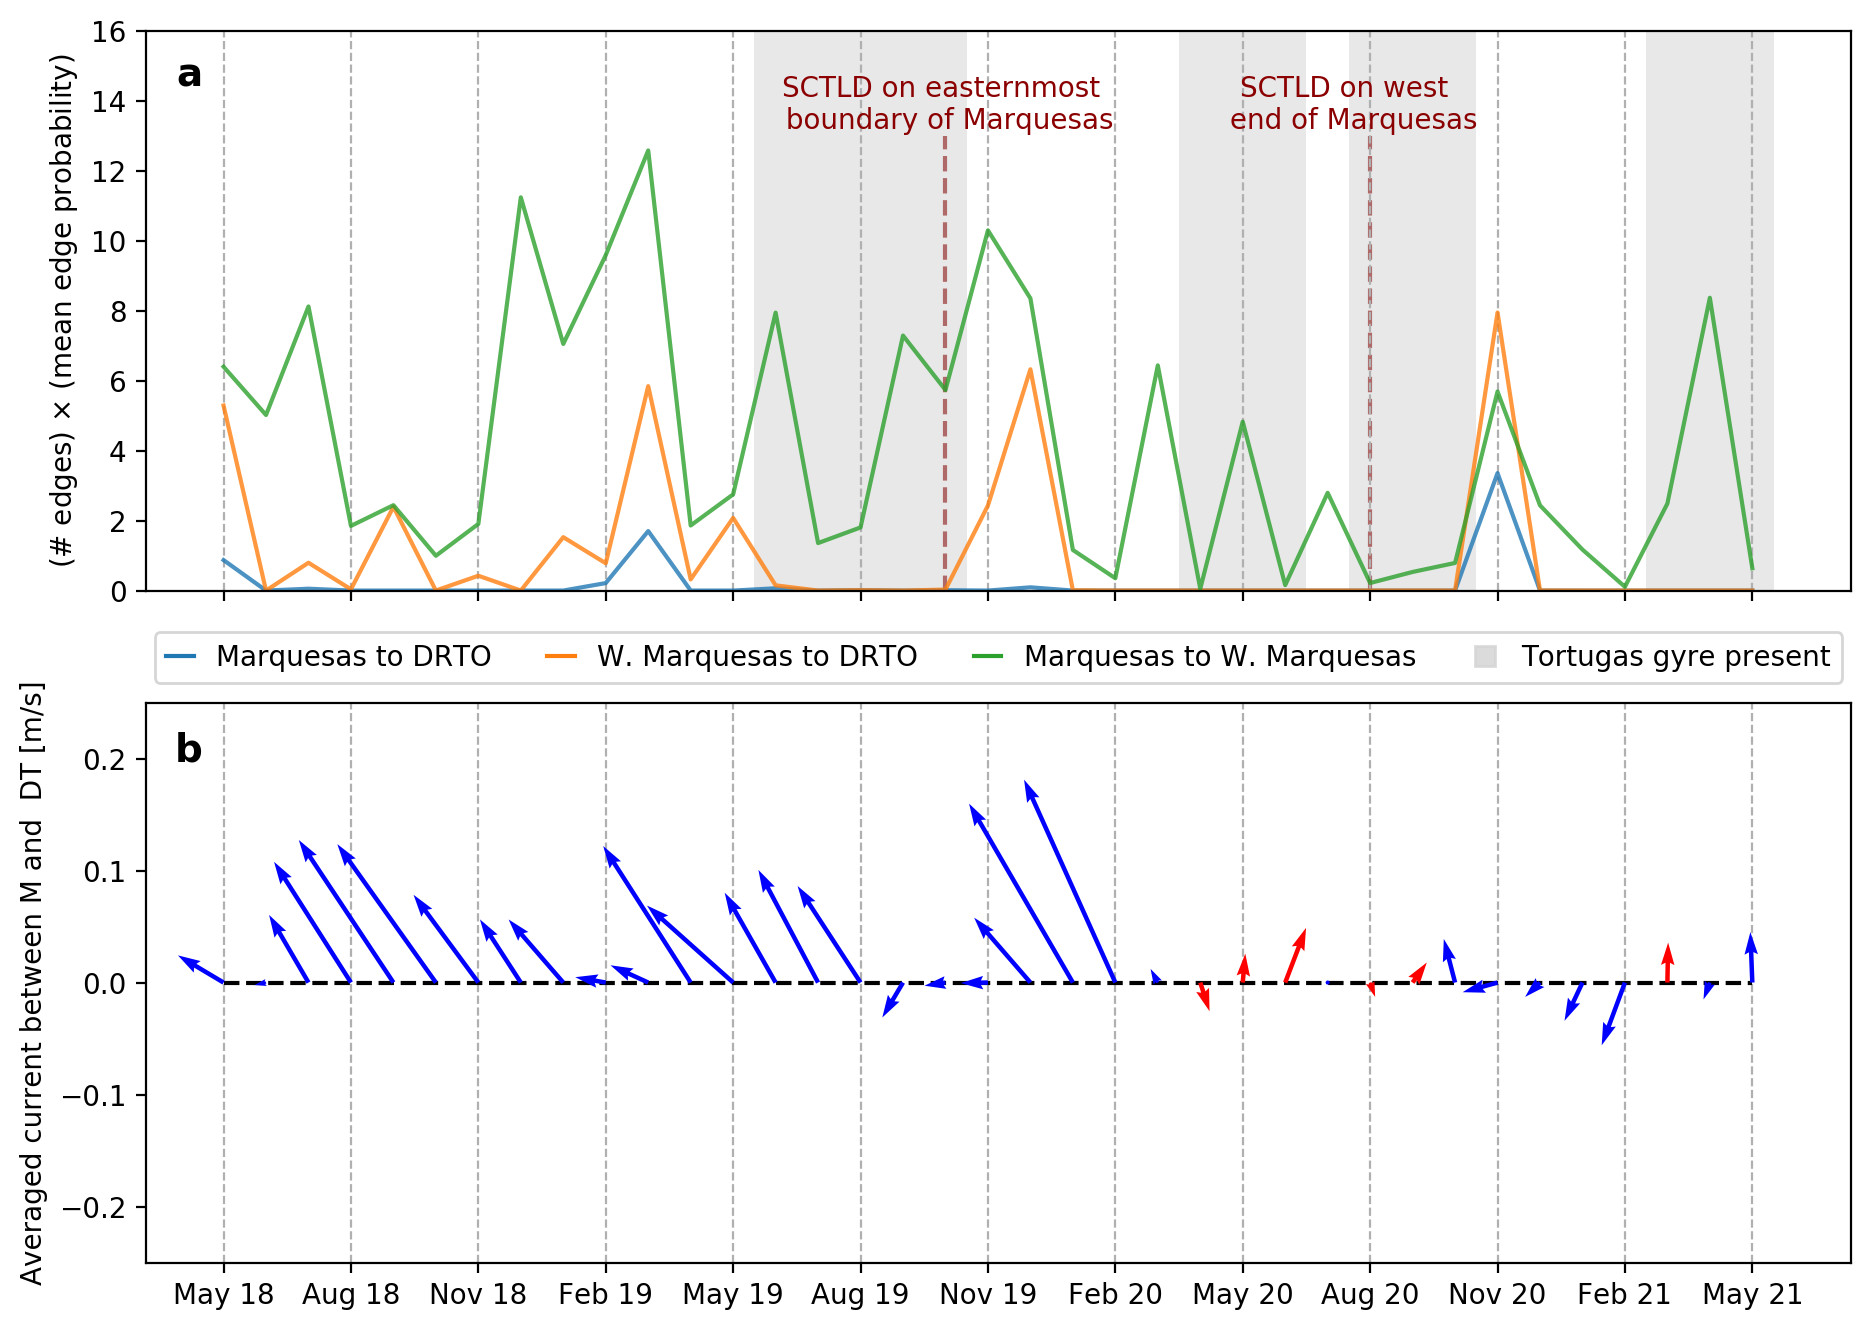
\includegraphics[width=.9\textwidth]{chapters/drto/figures/fig2.jpg}
    \caption{(a) Monthly connectivity indicator between the Marquesas and the DRTO (blue), the Western Marquesas and the DRTO (orange) and the Marquesas and the Western Marquesas (green) between May 2018 and May 2021. Months during which Tortugas gyres were observed in the ocean model outputs are highlighted in grey. Milestones of the observed propagation of the SCTLD through the Marquesas are indicated by dark red dotted lines. (b) Monthly mean currents between the Marquesas and the DRTO between May 2018 and May 2021. Mean ocean circulation with an eastward component is highlighted by red arrows.}
    \label{fig:fig2_drto}
\end{figure}

We analyzed the spatial patterns of hydrodynamic-predicted disease connectivity to the DRTO in November 2020 in more detail as the model suggested this was the month with the highest transmission probability due to high hydrodynamic connectivity. The most probable pathways to the DRTO originated mainly from southern reefs located between the Marquesas and the Western Marquesas, as well as from reefs of the northwestern end of the Western Marquesas (Fig. \ref{fig:fig3_drto}). This suggests that sub-reefs of these areas were more likely to send disease agents to the DRTO in November 2020. Conversely, no connection with large probability originated from the southwestern tip of the Western Marquesas, suggesting that they had very low potential to spread the disease to the DRTO. \\
The reefs with the highest vulnerability indicator value in November 2020 were mostly located on the eastern part of the DRTO, suggesting that these reefs were more likely to be affected during this month (Fig. \ref{fig:fig4_drto}a). More specifically our results suggest that an area of higher vulnerability was present in the vicinity of the locations where SCTLD was observed in May 2021. Vulnerability was the lowest on inner sub-reefs of the DRTO as they are not directly connected to the reefs of the Western Keys. This suggests that the disease must first spread through the outer reefs to reach them. The source indicator values confirm that disease transmission to the DRTO is more likely to originate from southern reefs at the interface between the Marquesas and the Western Marquesas, and reefs on the northwestern end of the Western Marquesas (Fig. \ref{fig:fig4_drto}b).

\begin{figure}
    \centering
    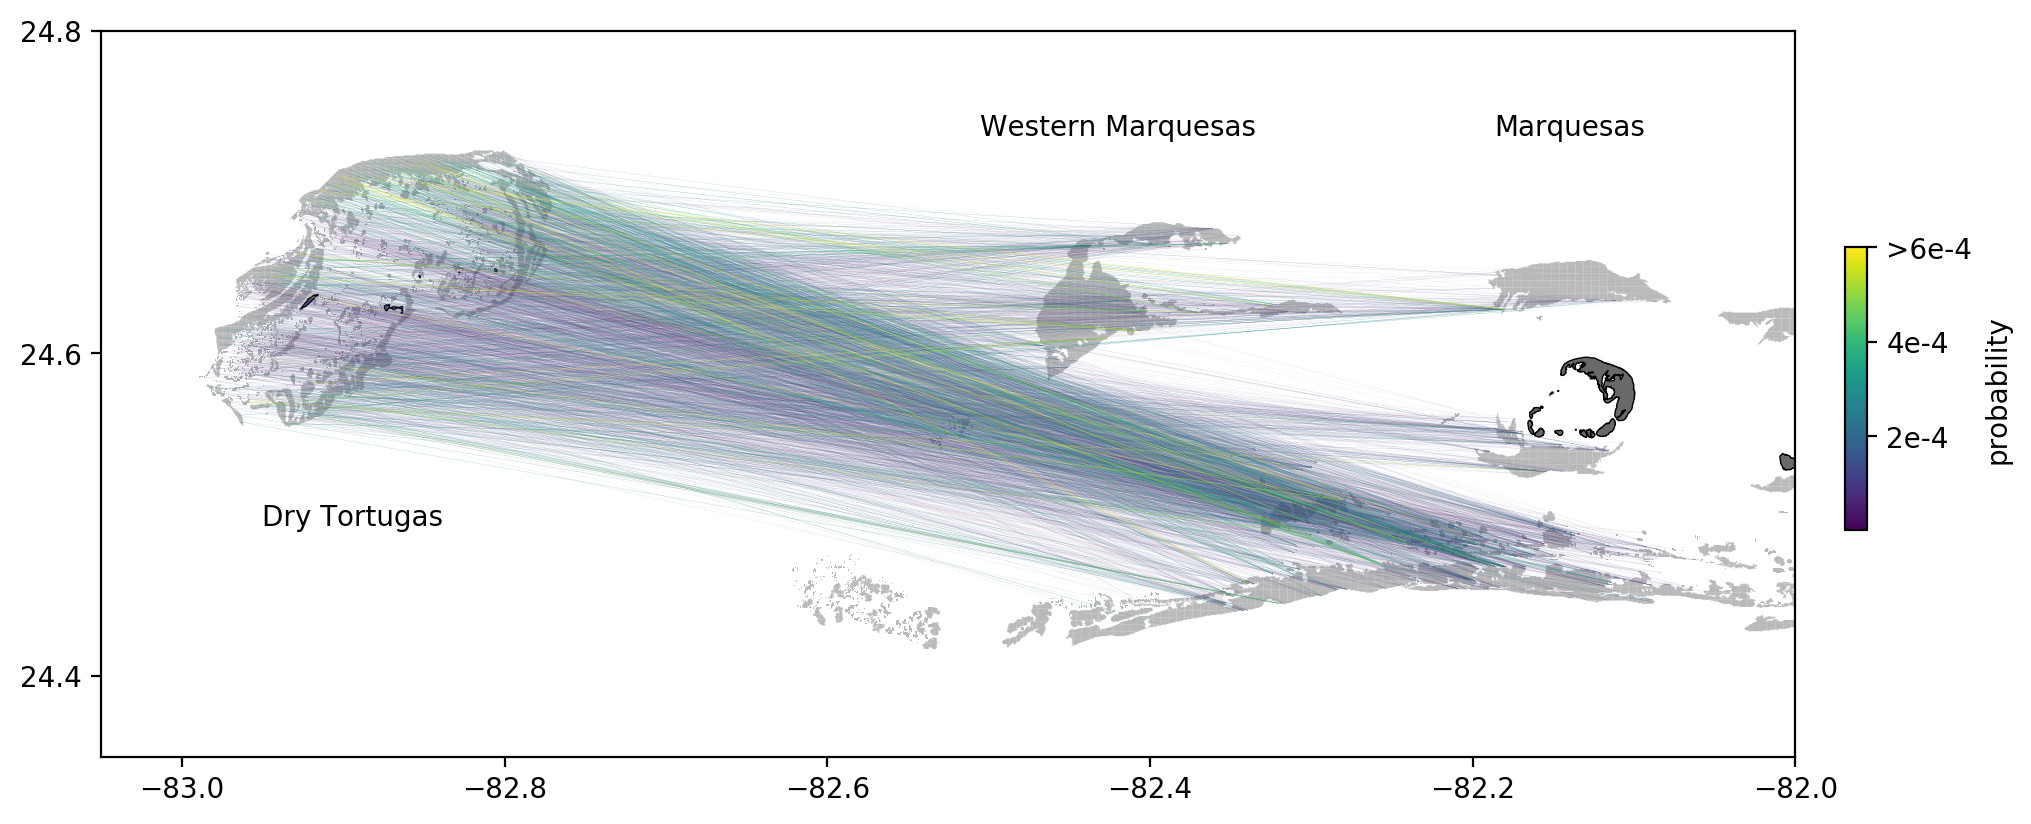
\includegraphics[width=.9\textwidth]{chapters/drto/figures/fig3.jpg}
    \caption{Edges with largest connection probability to each sub-reef of the DRTO from the Marquesas and the Western Marquesas in November 2020. Connections mostly originated from the southern reefs between the Marquesas and Western Marquesas, and from the northwestern reefs of the Western Marquesas. Reefs are highlighted in light gray while islands are shown in dark gray.}
    \label{fig:fig3_drto}
\end{figure}

\begin{figure}
    \centering
    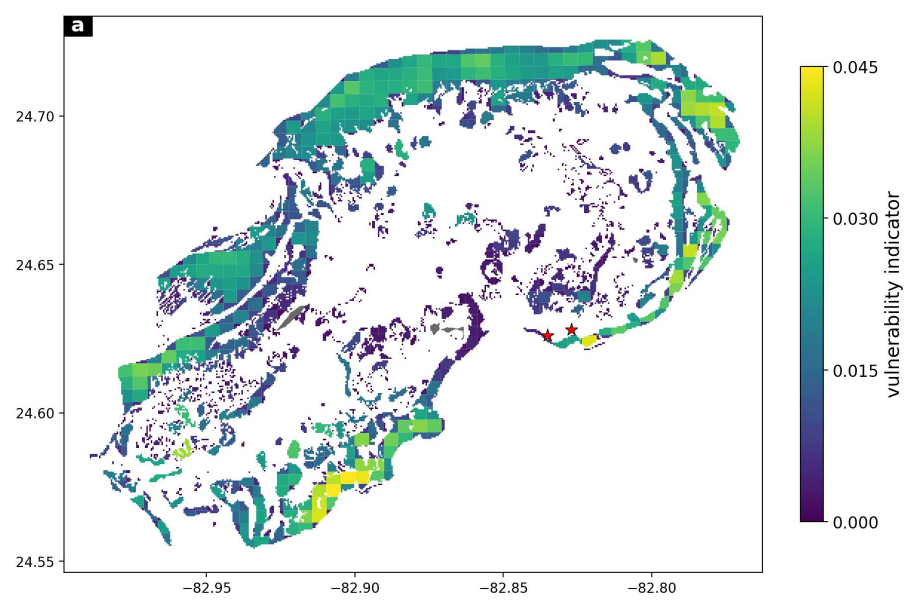
\includegraphics[width=.6\textwidth]{chapters/drto/figures/vulnerability_new.png}
    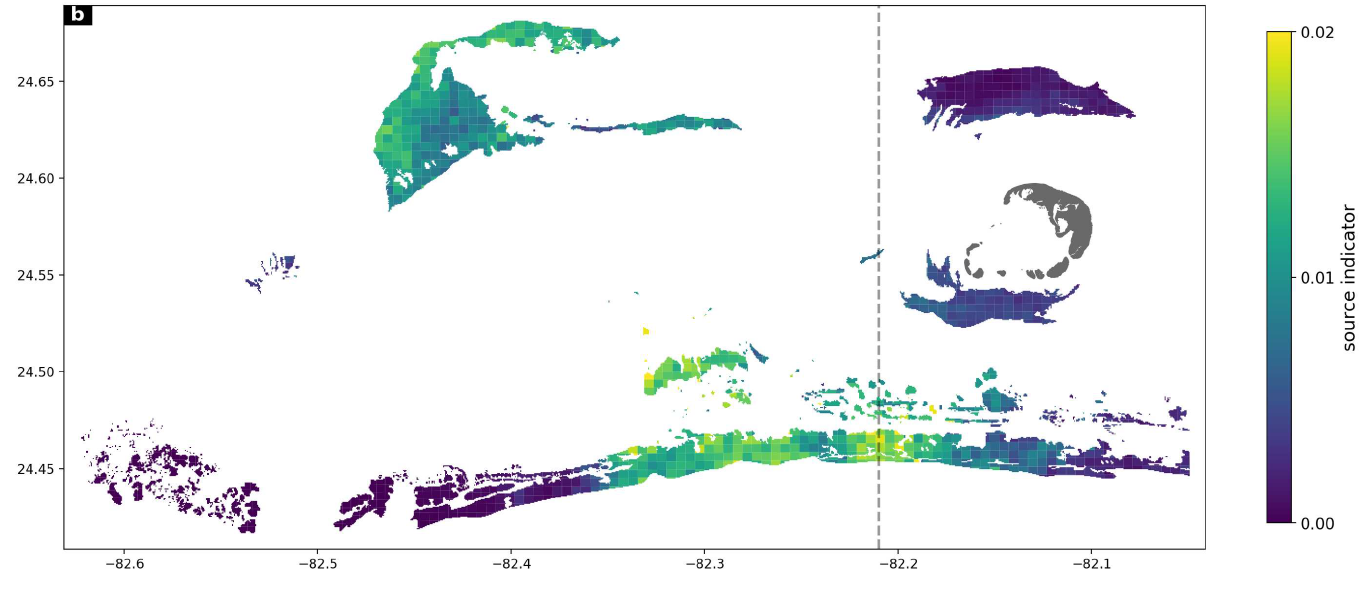
\includegraphics[width=.9\textwidth]{chapters/drto/figures/source_new.png}
    \caption{ (a) Vulnerability indicator value of all sub-reefs of the DRTO in November 2020. Eastern reefs of the DRTO appear most vulnerable to the disease. Locations where the SCTLD was observed in the DRTO are indicated by red stars (b) Source indicator value in November 2020 for every sub-reef of the Marquesas and the Western Marquesas. Northwestern reefs of the Western Marquesas and southern reefs between the Marquesas and the Western Marquesas show a higher transmission potential to the DRTO. Main islands are shown in dark grey, separation between the Marquesas and the Western Marquesas is indicated by a dashed line.}
    \label{fig:fig4_drto}
\end{figure}


\section{Discussion and conclusion}
Our results show that the eddies generated by the LC/FC system strongly influence the connectivity between the Marquesas and the DRTO. Mesoscale eddies modify the westward coastal currents by breaking them through strong cross-shore flow regime \citep{kourafalou2012florida}, as illustrated for October 2020 in Fig. \ref{fig:fig1_drto}. \cite{lee1994evolution} hypothesized that such cross-shore flow could impact the transport of larvae spawned in the Florida Keys and cause their retention on the West Florida Shelf for periods on the order of 6 months. As Tortugas eddies may remain stationary near the DRTO for up to 120 days \citep{fratantoni1998influence}, they may thus act as barriers for the exchanges between the Marquesas and the DRTO for extended periods of time. Moreover, the passage of mesoscale eddies was identified as one of the physical mechanisms likely to deliver larvae from the DRTO to the Upper Keys, therefore opposing exchanges from the Marquesas to the DRTO. Our results confirm the role of mesoscale eddies as potential barriers to connectivity between these two regions as most months during which Tortugas eddies were present correspond to a vanishing connectivity indicator. The fact that no eddies were observed at the beginning of our simulation might be related to the identification method, based solely on visual assessment of the residual currents. \modif{Alternative methods to identify the presence of eddies could have been the computation of the Okubo-Weiss parameter \citep{okubo1970horizontal,weiss1991dynamics} or the extraction of the FC position as the 20$^\circ$C isotherm at 150 m from HYCOM temperature fields, following the approach of \cite{kourafalou2012florida}}. A comprehensive identification of all Tortugas eddies during our simulated period would require the analysis of sea surface temperature and elevation, which is beyond the scope of the present study. . While our approach might miss some Tortugas gyres, it filters out submesoscale eddies with lifespan of the order of several days. Consequently, when horizontally elongated mesoscale cyclonic streamlines are present in the computed monthly-averaged currents, they can be identified as Tortugas eddies with sufficient certainty.

The connectivity from the Marquesas to the DRTO does not seem to follow any clear seasonality and exhibits high interannual variability. Although a longer simulation period might be required to rigorously assess the presence of seasonal variations, no clear seasonal patterns were observed over the 3-year simulated period for both the connectivity indicator and the mean currents (Fig. \ref{fig:fig2_drto}). In this regard, the boundary of the West Florida Shelf significantly differs from the inner shelf, which exhibits a robust cycle between summer and winter months \citep{liu2012seasonal}. Furthermore, our results indicate that the connectivity from the Marquesas to the DRTO strongly varies from year to year. This is best illustrated in March-September 2020, during which no connectivity was observed for an extended period of time and the dominant currents between the Marquesas and the DRTO had an eastward component. Such behavior was not observed during the rest of the simulation. These results are consistent with the strong variability of the LC/FC system, which strongly impacts circulation near the DRTO. \cite{lee1994evolution} and \cite{fratantoni1998influence} first described the influence of the LC penetration and ring shedding dynamics in the GoM on the formation of eddies near the DRTO. \cite{kourafalou2018physical} then further identified that LC eddy separation events were related to the formation of southward currents over the Pulley Ridge reefs and the perturbation of the slope stratification on the Southwestern Florida Shelf. The detachment of anticyclonic eddies from the main LC affects in turn the position of the FC, which strongly impacts eddy activity near the DRTO and the Marquesas, either through the formation of local eddies or the retention of remote eddies near the DRTO \citep{kourafalou2012florida}. These variations of the FC position have been shown to have no seasonal pattern with strong interannual variability and generate complex eddy to eddy interactions \citep{kourafalou2012florida}. Furthermore, the DRTO area was identified as a region of significant importance for the ecology of the West Florida Shelf, as contacts with the LC cause the inflow of nutrients that modify water properties on the shelf \citep{weisberg2003local,liu2016offshore}. \cite{weisberg2017loop} further hypothesized that these contacts might in turn impact the penetration of the LC in the GoM.

We have shown that the ocean circulation, and in particular the presence or absence of eddies shed from the Florida Current, coincides with the timing of initial SCTLD observations and likely transmission to the DRTO. However, it is important to note that it is currently not possible to determine whether SCTLD is caused by a novel pathogenic agent or simply a variant of a previously existing disease that causes tissue loss on corals. The DRTO has experienced episodic outbreaks of tissue loss in years prior to 2020 (see \citealp{frrp2018}). These previously documented tissue loss events occurred during the summer months within isolated reef sites and primarily affected one genus of corals, \textit{Orbicella}. Although the ecology of SCTLD documented from 2014 to the present differs from these previous reports, until pathogenic agents are identified, the positive identification of a particular coral disease, such as SCTLD, will remain presumptive. However, past studies indeed suggest SCTLD is likely caused by a waterborne agent regardless of the particular pathogen at play. As such, intense eddy activity between February 2020 and May 2021 would have largely prevented the exchange of disease agents westward, with the exceptions of November and December 2020. During those two months, the residual circulation on the southwestern Florida shelf turned westward, and thus would have allowed disease agents to reach the DRTO. The transmission of disease agents to the DRTO was most likely to occur in November 2020, when the connectivity indicator was the largest. The developed vulnerability indicator indicates that sub-reefs on the eastern part of the DRTO were more likely to be affected by the disease. These results are consistent with observation as the locations where SCTLD was observed in the DRTO are located near sub-reefs identified as highly vulnerable by our model \citep{kramer2019map}. Nonetheless, the area predicted to be vulnerable exceeds the extent of the region where signs of the disease were first observed. These discrepancies might be explained by the fact that our vulnerability indicator accounts for all potential connections to a given sub-reef. In practice, these connections only yield the transmission of disease agents if the sub-reef they originate from is affected by SCTLD. Our model might therefore overestimate the vulnerability of some sub-reefs. Moreover, due to the lack of data on coral distribution in FCR, an uniform coral density was assumed over all reefs. The impact of some reefs with low coral cover might thus be overestimated by the model. Nonetheless, we argue that our model remains a valuable tool to assess the (absence of) connectivity between the Marquesas and the DRTO.
 
Model results suggest a time lag of 5 to 6 months between the moment the hydrodynamics predicted that disease agents reached the DRTO and the moment SCTLD symptoms were observed in the DRTO. This seems to contradict the results of previous modeling and experimental studies that found SCTLD transmission times of 10 days or less \citep{dobbelaere2020coupled, meiling2021variable}. However, several elements might explain a slower development of the disease on the DRTO. First, in situ conditions might significantly differ from the ones of a controlled tank environment, potentially leading to differences in the time required for the first disease lesions to appear. Furthermore, disease transmission in the Florida Keys might occur faster as reefs can receive disease agents from several affected neighboring reefs. In the case of disease agents reaching the fully susceptible population of the DRTO, such interactions with neighboring affected colonies do not take place and the outbreak might therefore require more time to develop. Furthermore, our results suggest that corals of the DRTO could only be exposed to agents coming from the Marquesas in November and December 2020, while exposure to incoming disease agents was continuous in the Keys due to the density of the reef system. Additionally, the epidemiological parameters of \cite{dobbelaere2020coupled} were calibrated on species-averaged prevalence data in the Florida Keys, which might not be representative of the colony composition and environmental conditions in the DRTO. Finally, observational data is dependent on the frequency and spatial distribution of field missions and might therefore give an incomplete picture of the situation on the field. For example, fine scale observations of SCTLD in the Lower Florida Keys found low disease incidence (< 10 colonies) starting in October, and then disease incidence peaked in April 2019 \citep{williams2021fine}. Alternatively, one might argue that this lag between the modeled transmission of the disease agents to the DRTO and the first observations of the SCTLD indicates that the propagation of the disease was not caused by local currents. In that case, another vector, such as ballast waters, might have to be considered. However, such investigations are beyond the scope of the present study.

It is important to note that the time and location of the first observations of an outbreak do not necessarily correspond to its initiation. An epidemic might grow unnoticed during its first stages, as it first develops at a linear rate before growing exponentially. Tools such as the ones developed in the present study might therefore have helped to mitigate the SCTLD during the first stages of its development in the DRTO, before May 2021. Furthermore, this study has shown that strong eddy activity near the DRTO was likely to interrupt connectivity from the Western Florida Keys to the DRTO. Therefore, monitoring eddy activity through satellite observations of sea surface temperature and sea surface elevation anomaly \citep{kourafalou2018physical} might serve as a proxy for reef managers to estimate connectivity between these two areas. The implications of our connectivity results are not limited to the propagation of disease agents and apply to the spread of any type of propagules from the Marquesas and the DRTO. This study therefore brings additional insight on the physical and environmental connectivity in the southwestern part of FCR.

\begin{subappendices}
	\section{Validation of the model}\label{drto:validation}
	
	SLIM outputs were validated against field measurements from tide gauges and ADCP in the Florida Keys and on the shelf (Fig. \ref{fig:a1}). Here, we show the comparison between observed and simulated sea surface elevation and current speed for the month of November 2020. The model accurately reproduces the observed sea surface elevation at all tide gauges (Fig. \ref{fig:a2}) with an RMSE of less than 8 cm. The current velocity on the shelf is also  well reproduced by the model, despite a slight underestimation of the southward component of the observed currents at mooring C10 and C22, located on the 25 m and 70 m isobaths respectively (Fig. \ref{fig:a3}). Using the vector correlation analysis of \citep{kundu1976ekman}, we obtained a correlation factor of 0.9 and a veering angle of 10$^\circ$ between the modeled currents and the observations at station C10. A correlation factor of 0.75 and a veering angle of 8° were obtained at mooring C22. Such values are similar to the performances of previous modeling studies on the West Florida Shelf \cite{liu2020impacts}.
		
	\begin{figure}
		\centering
		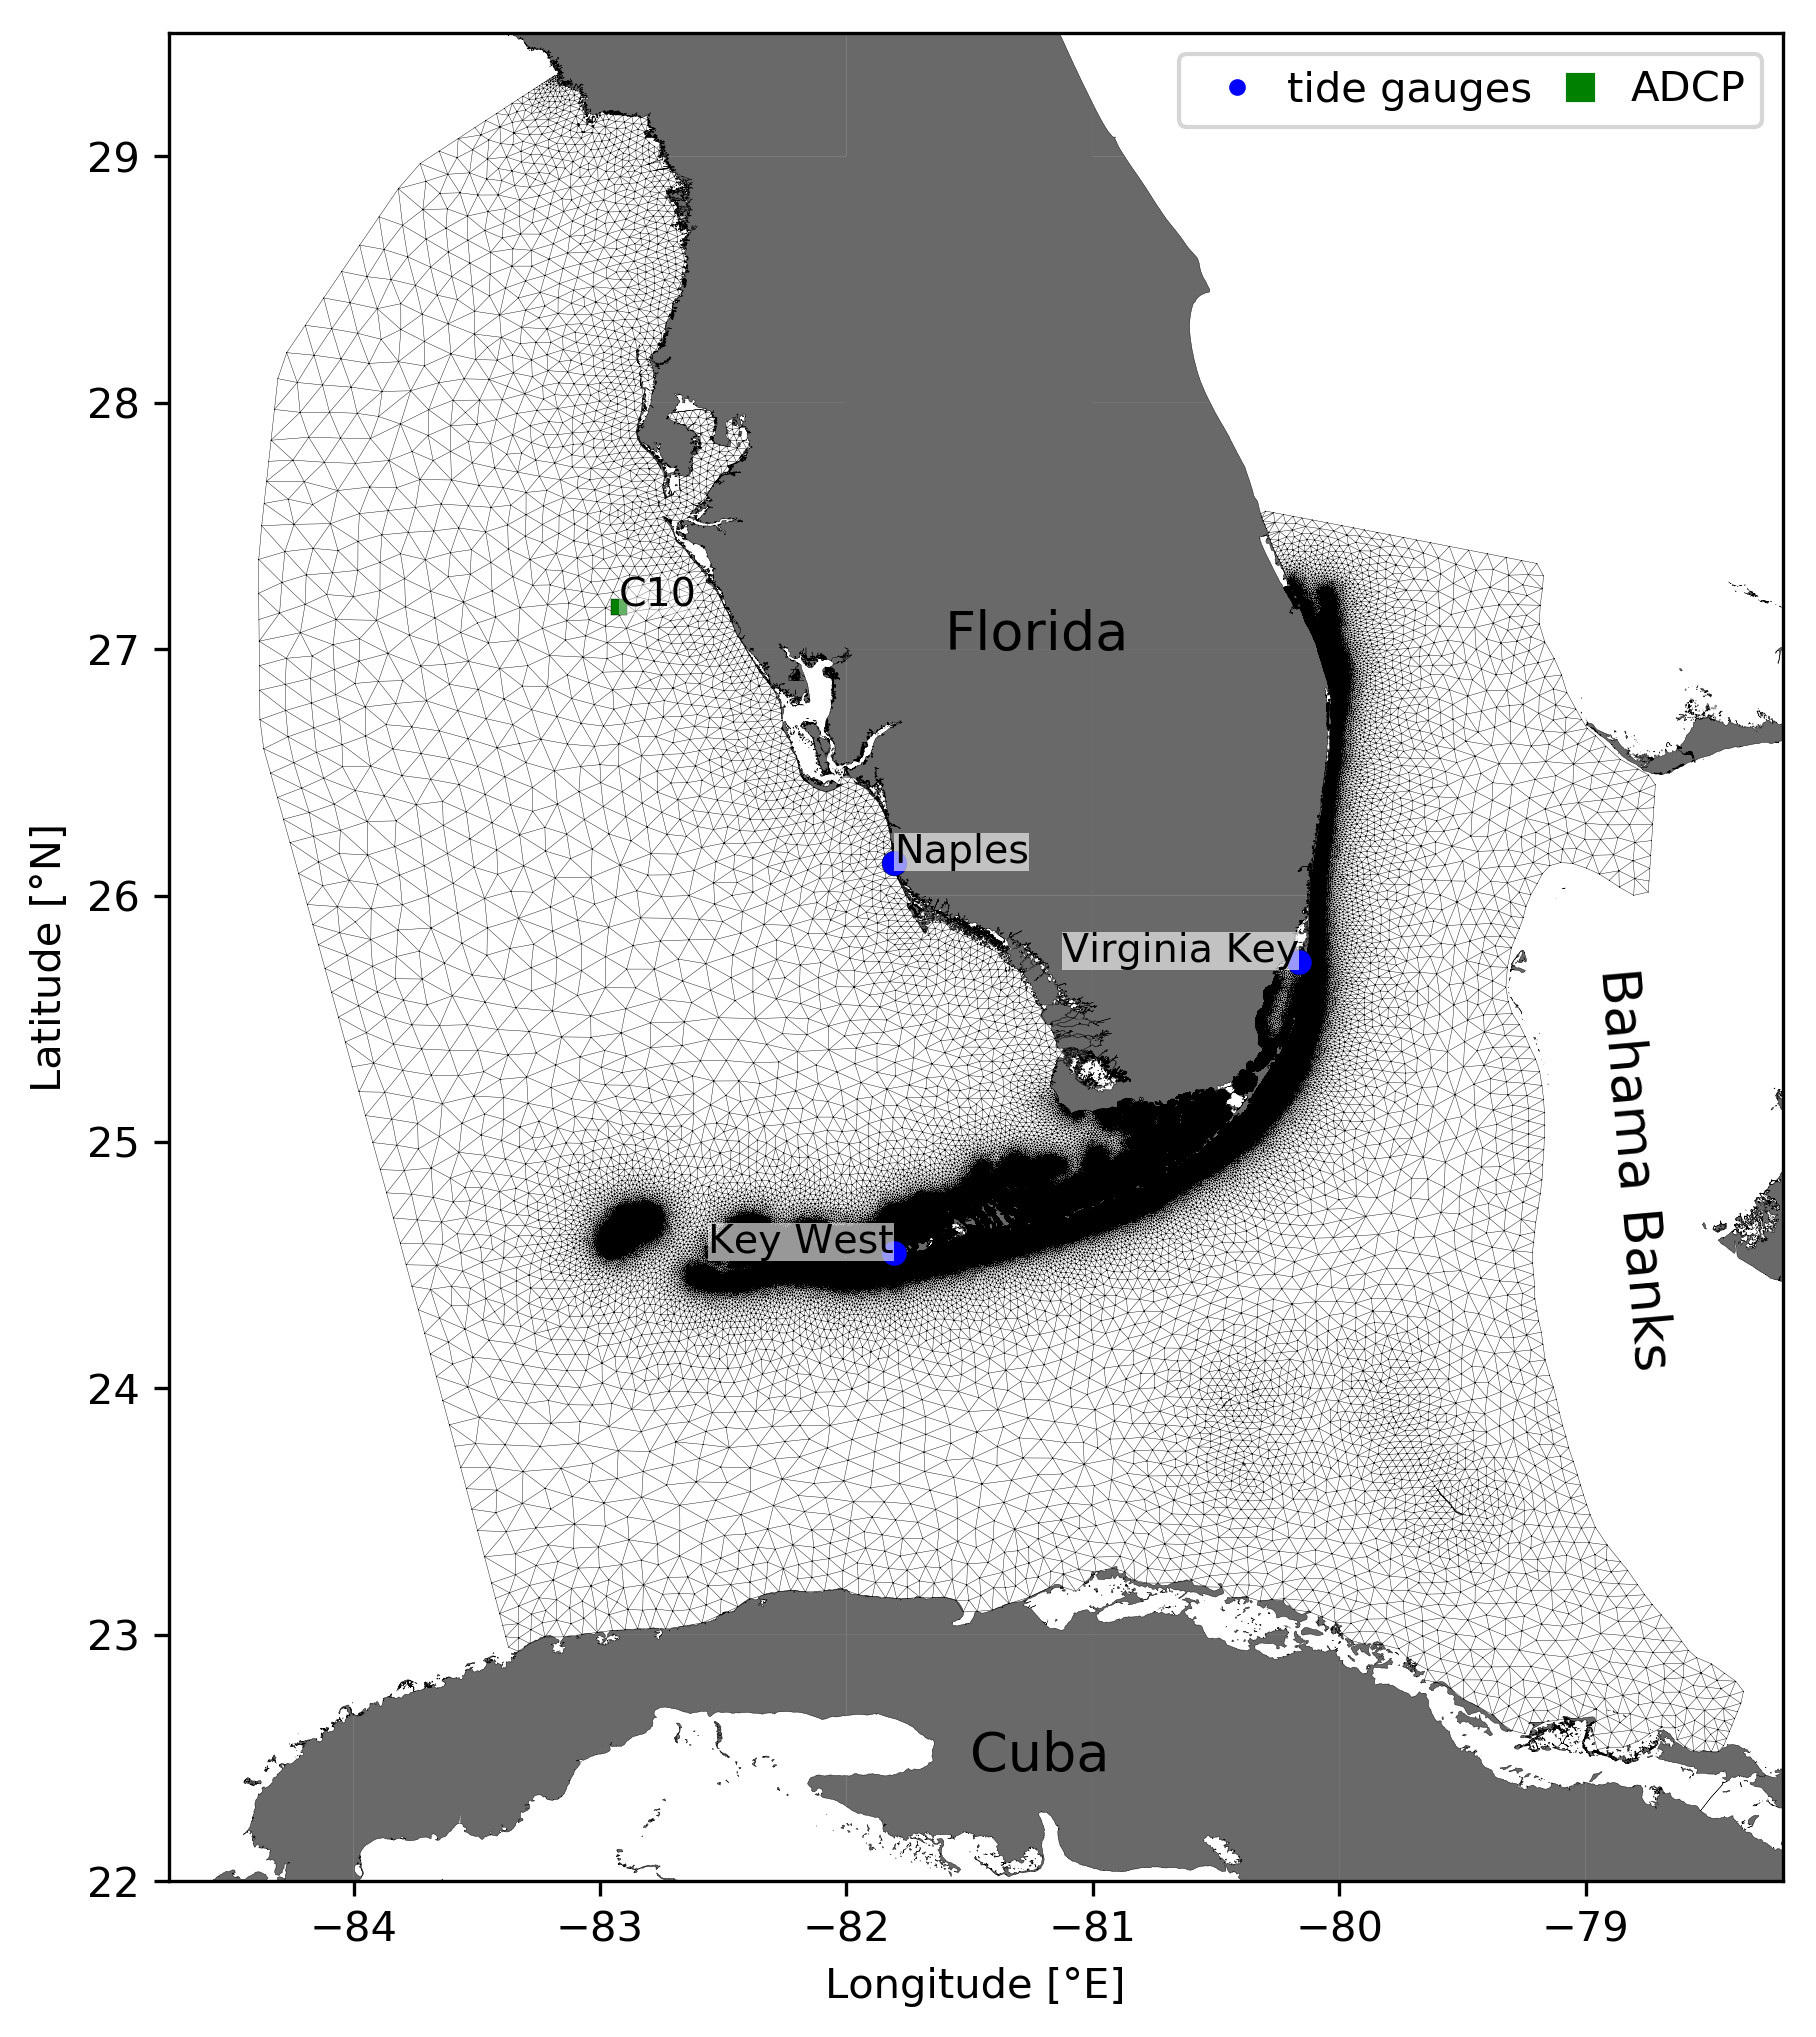
\includegraphics[width=.8\textwidth]{chapters/drto/figures/a1.JPEG}
		\caption{Mesh of the computational domain with the location of the stations used for the validation of the model outputs. Land is shown in dark gray.}
		\label{fig:a1}
	\end{figure}
	
	\begin{figure}
		\centering
		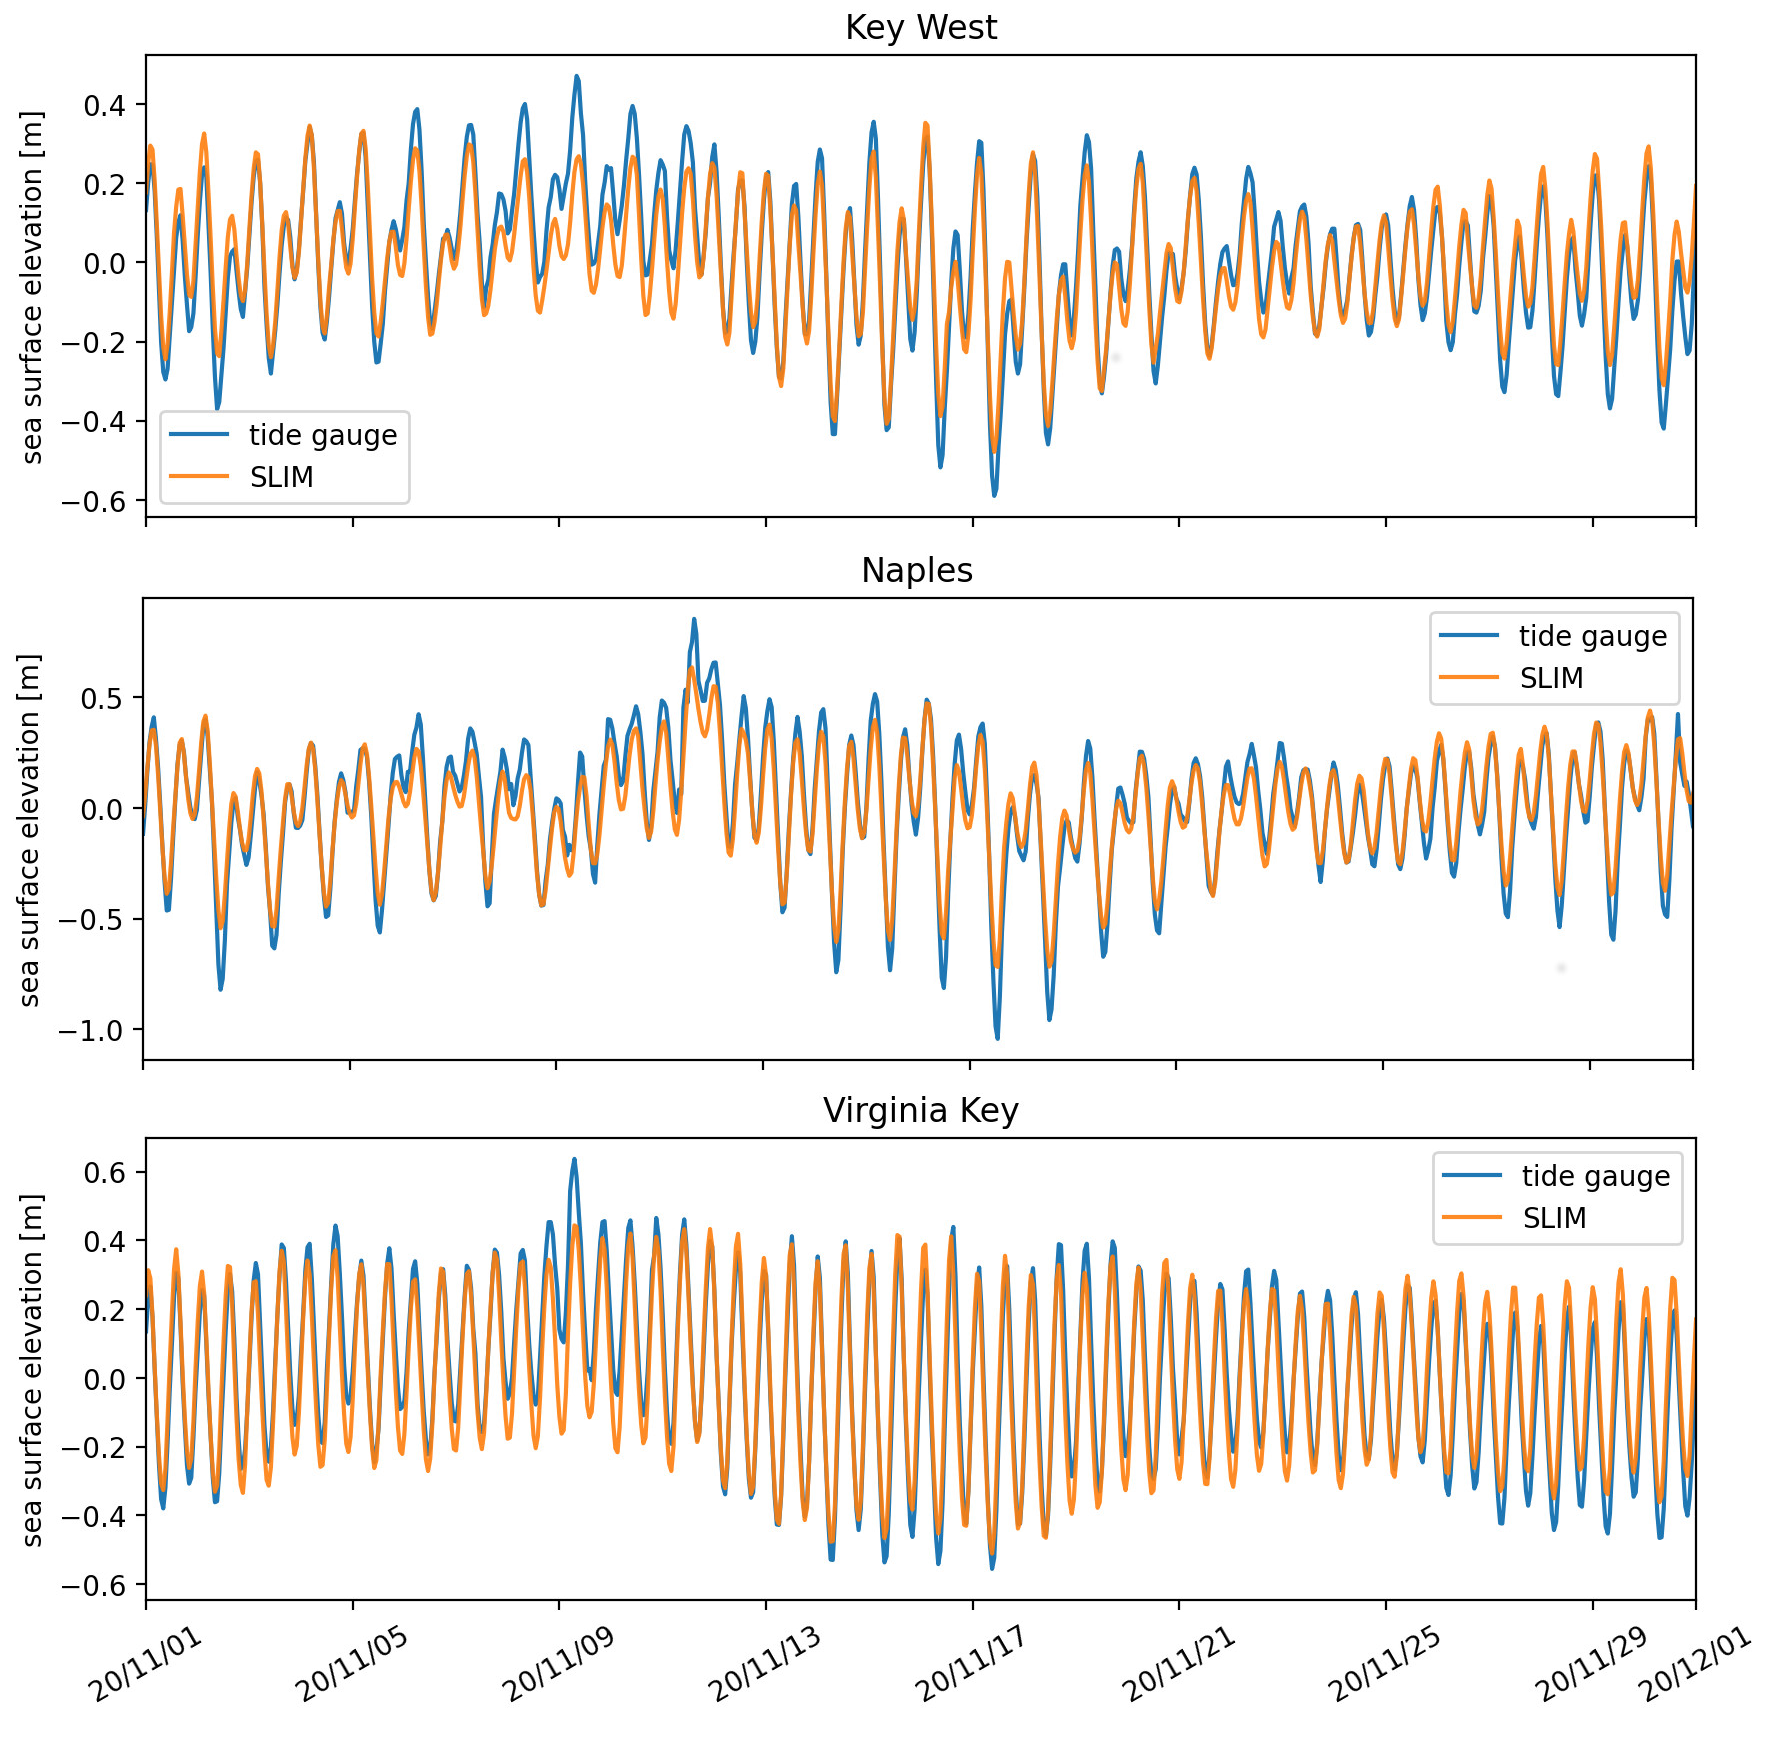
\includegraphics[width=\textwidth]{chapters/drto/figures/a2.png}
		\caption{Comparison of SLIM sea surface elevation against tide gauge elevation in November 2020. The tidal signal is well reproduced at all stations with an RMSE of less than 8 cm.}
		\label{fig:a2}
	\end{figure}

	\begin{figure}
		\centering
		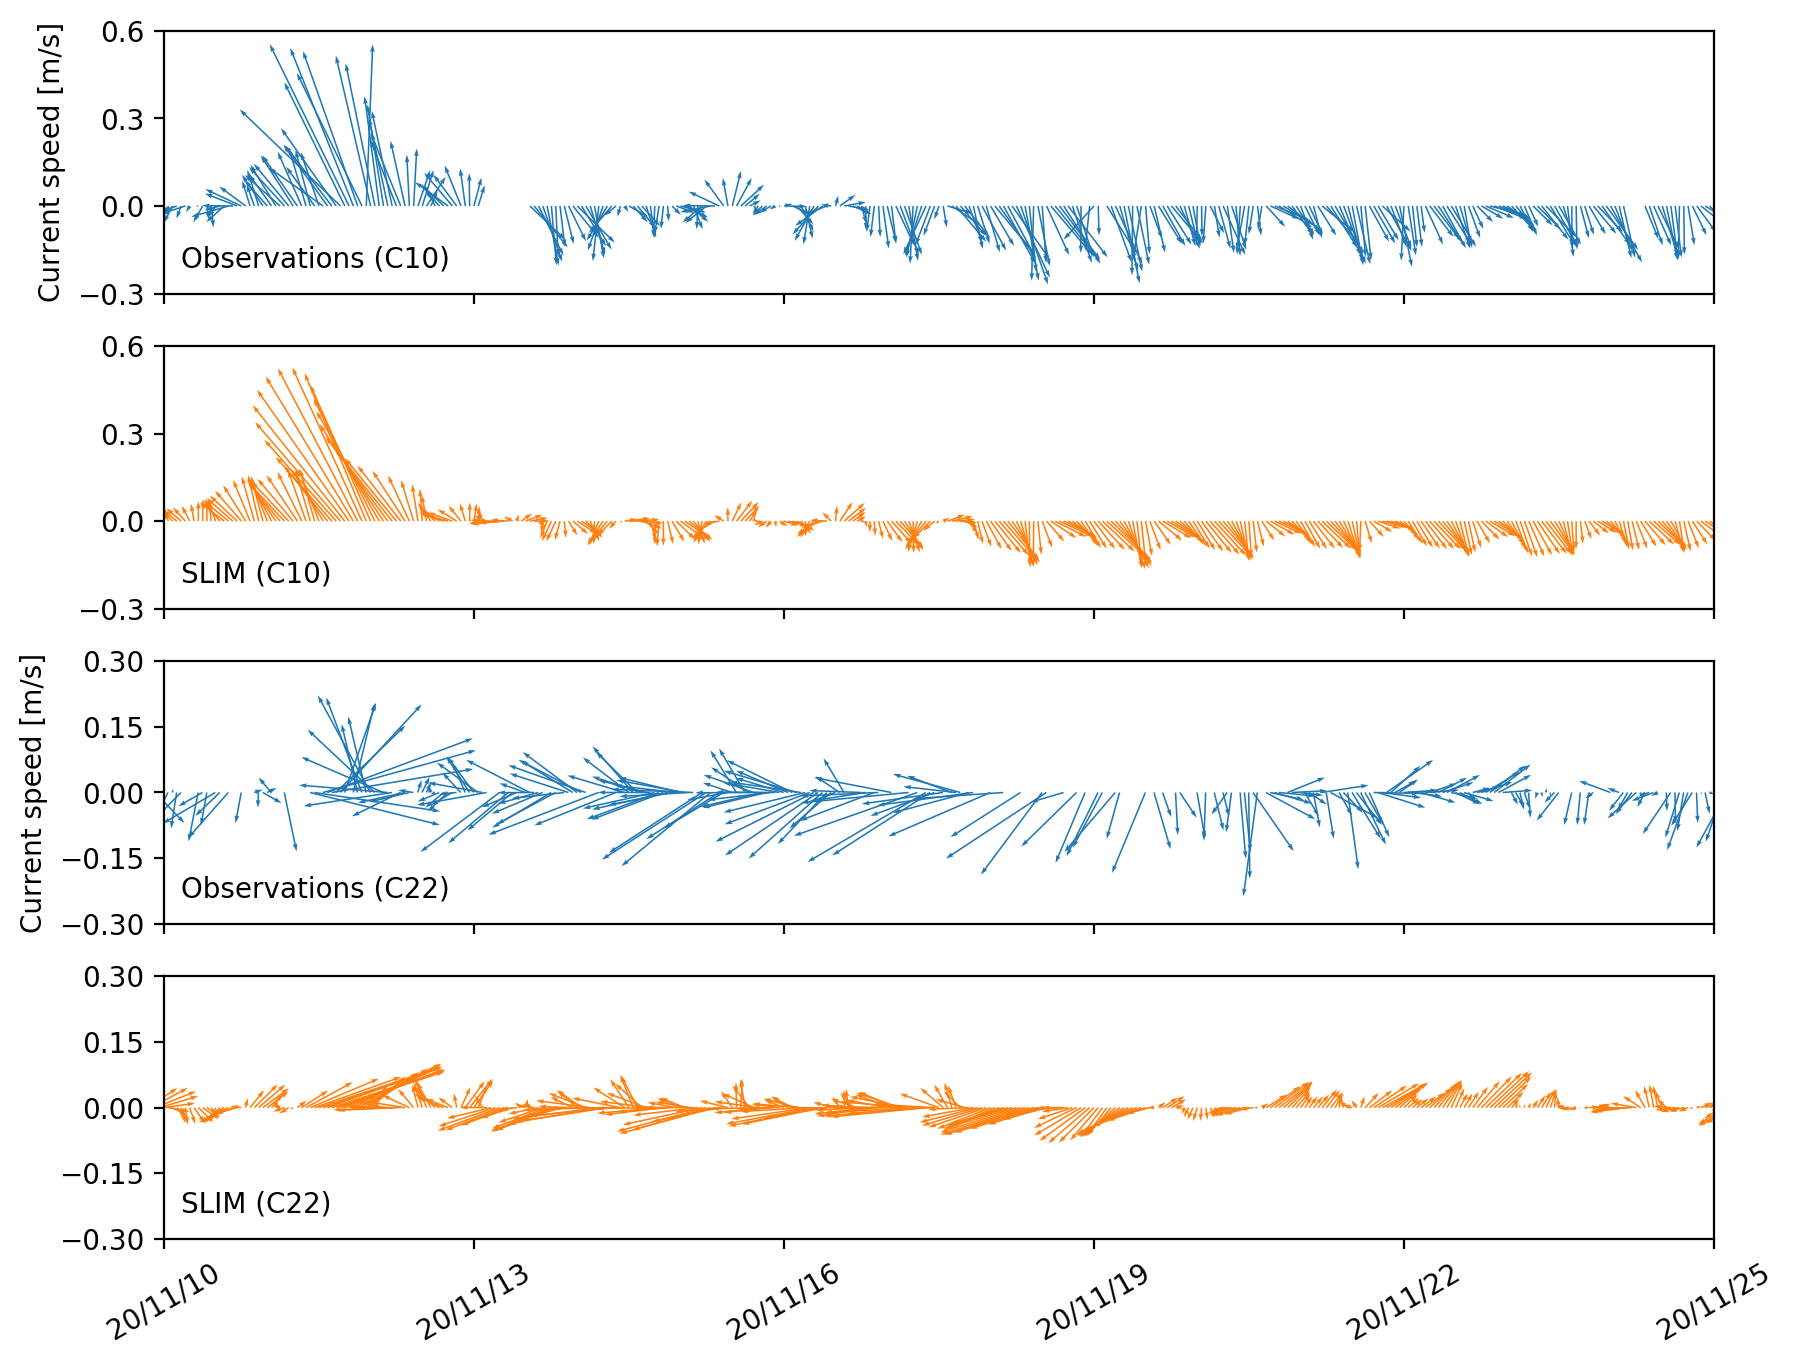
\includegraphics[width=\textwidth]{chapters/drto/figures/a3.png}
		\caption{Comparison of SLIM currents with depth-averaged ADCP measurements at mooring C10 and C22 in November 2020. Despite a slight underestimation of their southward component, currents and their oscillations are well reproduced by the model.}
		\label{fig:a3}
	\end{figure}
		
	SLIM relies on its coupling with HYCOM GoM to accurately reproduce the Loop Current (LC)-Florida Current (FC) system. HYCOM’s surface fields were therefore compared with sea surface temperature data from the Group for High Resolution Sea Surface Temperature (GHRSST; \url{https://www.ghrsst.org/}). HYCOM reproduces well the penetration of the LC in the Gulf of Mexico (Fig. \ref{fig:a4}), which is key to simulating the eddy activity linked to the meandering of the FC near the DRTO.
	
		\begin{figure}
		\centering
		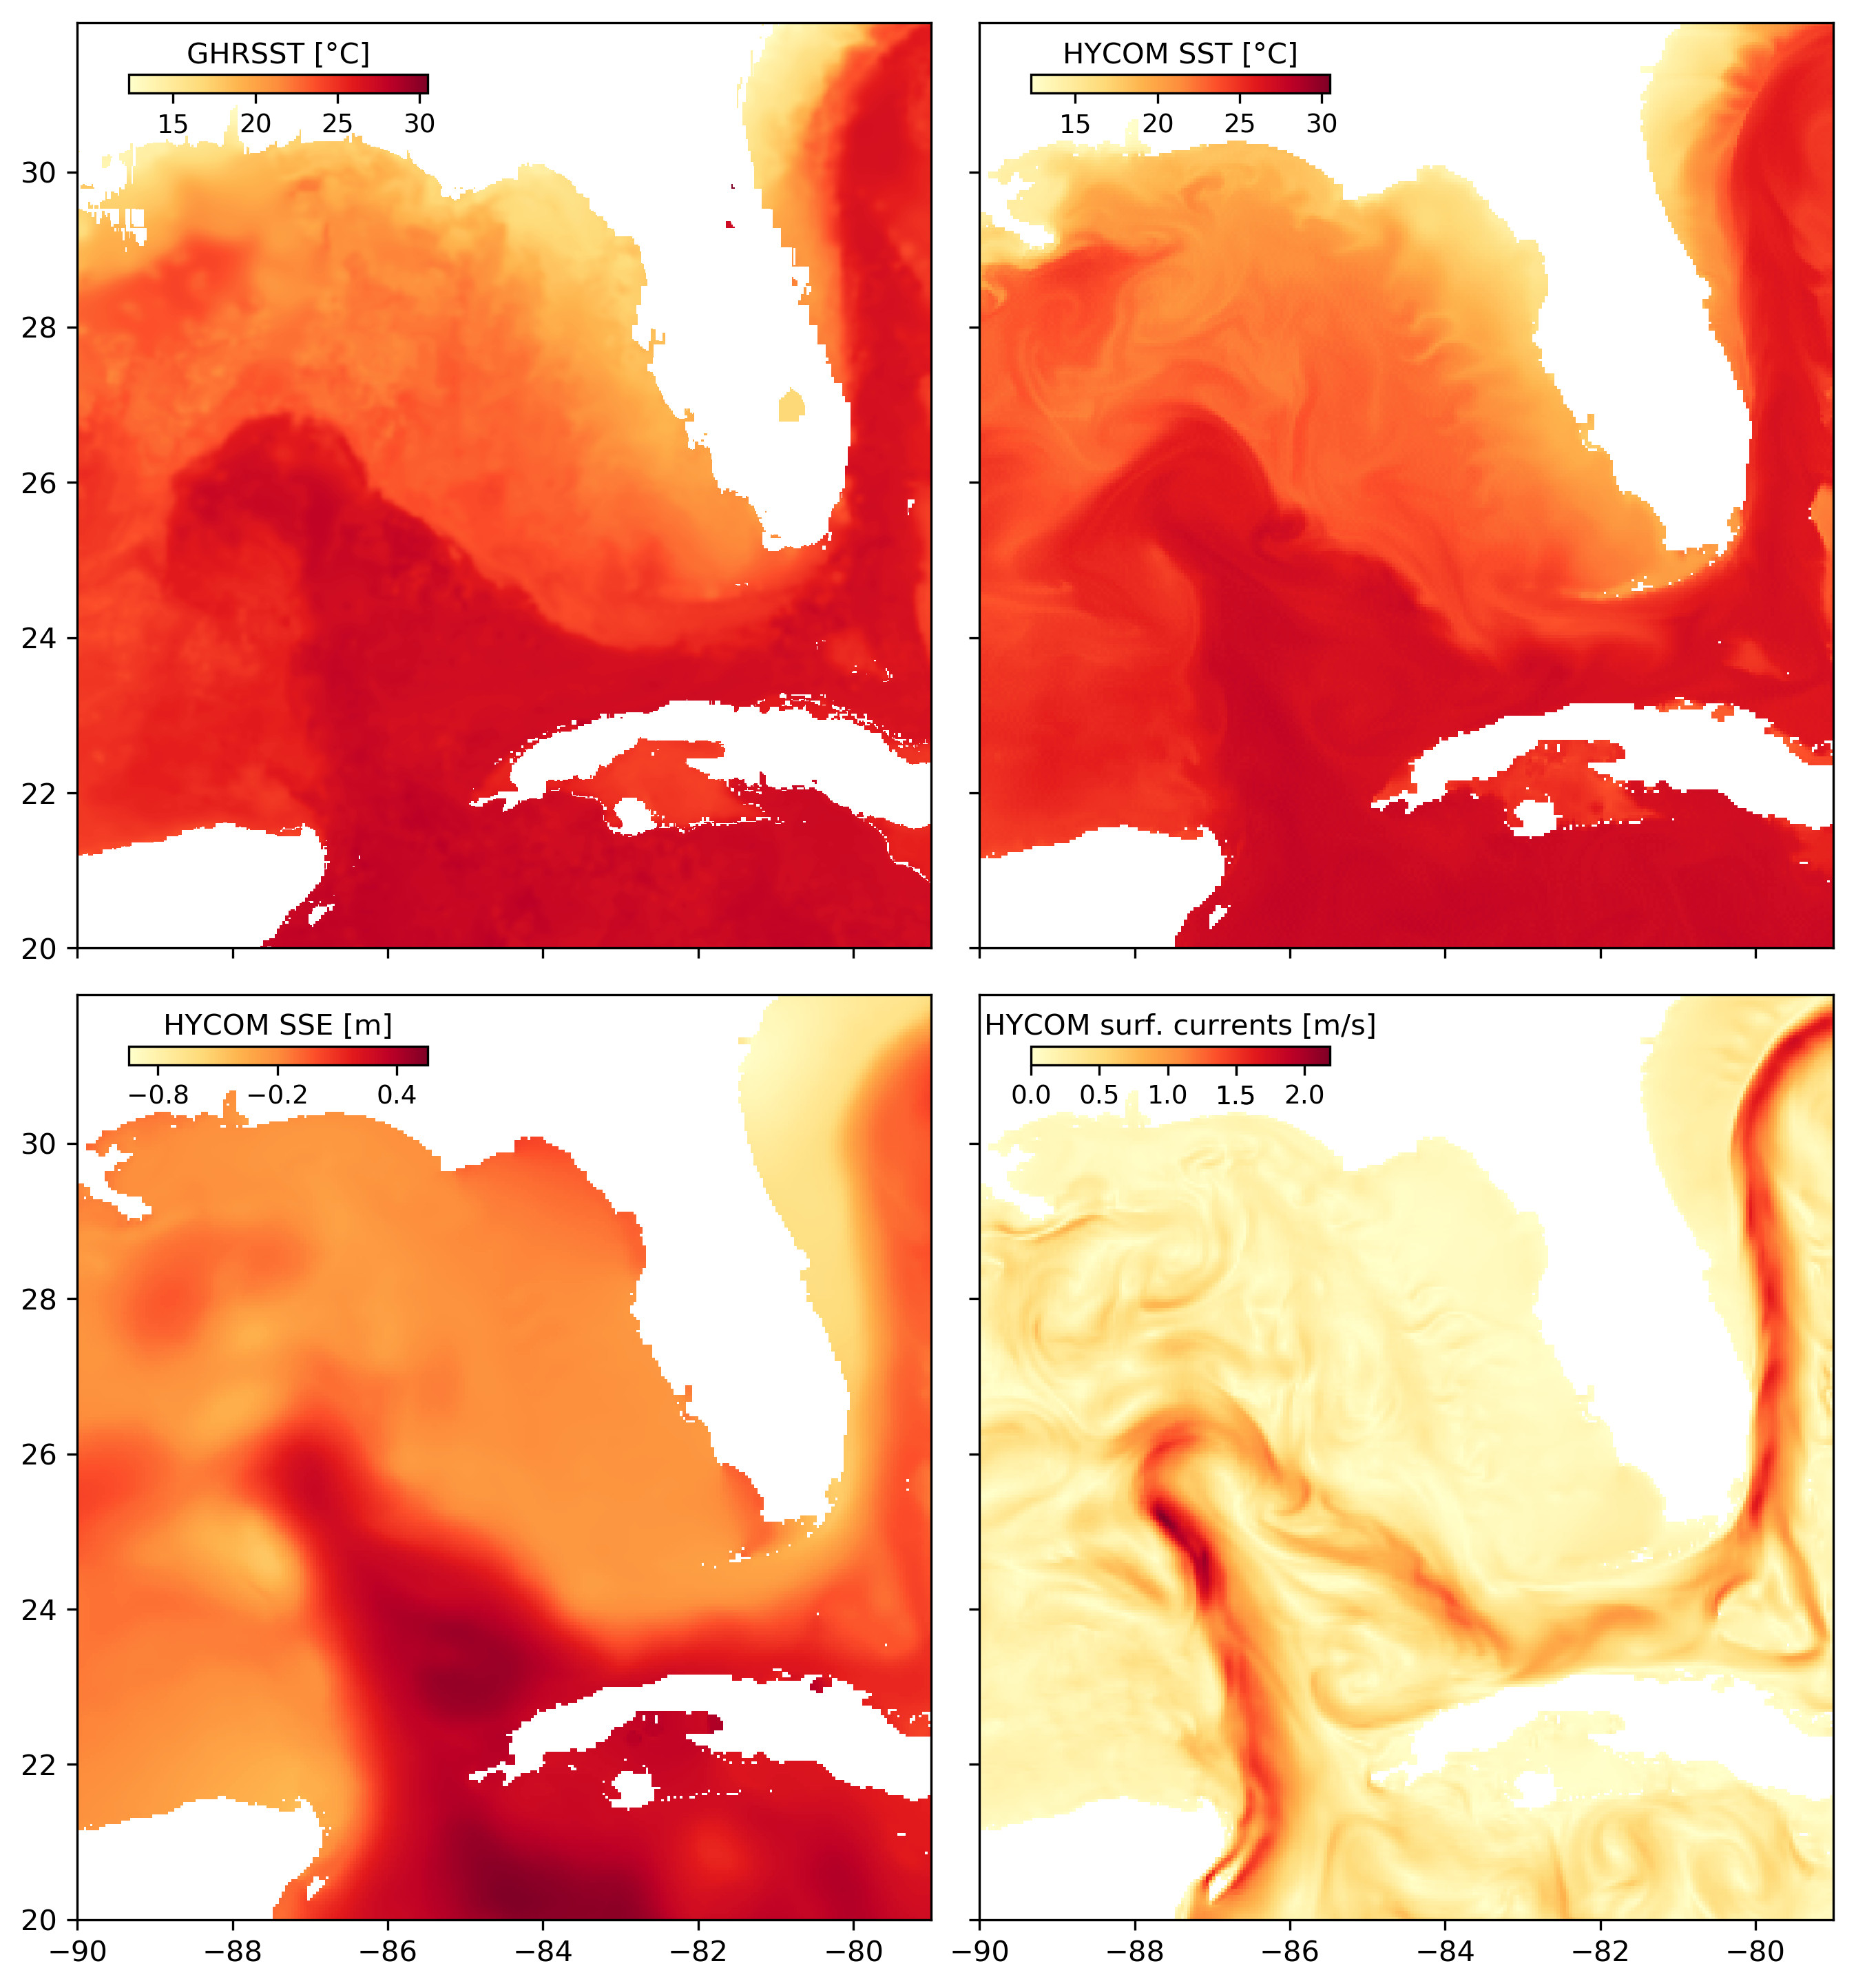
\includegraphics[width=\textwidth]{chapters/drto/figures/a4.JPEG}
		\caption{Comparison of (\textbf{A}) satellite-derived sea surface temperature from the Group for High Resolution Sea Surface Temperature (GHRSST) against (\textbf{B}) sea surface temperature, (\textbf{C}) sea surface height (SSH) and (\textbf{D}) surface current magnitude modeled by HYCOM. All panels are snapshots of November 15, 2019 at 0000 UTC.  The model reproduces well the penetration of the LC in the Gulf of Mexico.}
		\label{fig:a4}
	\end{figure}
	
\end{subappendices}